\documentclass[../rapport_MVEX01-11-05]{subfiles}
\begin{document}
\subsection{Klassificering}
En HMM behöver distinkta observationer för att fungera; dessa
observationer kommer vi att identifiera med hjälp av klassificering av
nyckelbilder ur videon utifrån ett antal egenskaper vi identifierar
med hjälp av den binära hudkartan för motsvarande bild.

Själva klassificeringen är mycket enkel. Vi utgår från ett vektorrum
av egenskaper, där varje egenskap representerar en dimension. I detta
vektorrum placerar vi ut nyckelbilder från förinspelade gester, genom
att för varje (nyckel)bild i videosekvensen beräkna alla egenskaper.
Efter detta gallras nyckelbilderna ut, så att de som ligger allt för
nära varandra tas bort, tills antalet nyckelbilder är tillräckligt
litet (cirka tio stycken).
Detta ger oss en slags kodbok vilken vi sedan kan använda för att
klassificera bilder från andra videosekvenser. 

\marginpar{Vikta vissa features?}

Detta görs genom att för varje bild beräkna en egenskapsvektor, som
sedan jämförs med de sparade vektorerna. Bilden klassificeras sedan
genom den nyckelbild som ligger närmst i egenskapsrummet enligt något
lämpligt mått (exempelvis det euklidiska avståndet). Detta gör att vi
får en stadig ström av heltal (en per bild i videosekvensen) som i
någon mening projicerar videosekvensen på mängden av sparade
nyckelbilder --- dessa heltal skickas sedan till en HMM som avgör om
videosekvensen faktiskt liknar den gest som definieras av dessa
sparade nyckelbilder.

\subsection{$k$-nearest-neighbour}

%Detta måste givetvis göras en gång per gest, vilket ger oss en kodbok
%per gest; detta eftersom vi har en HMM per gest.
%
%\marginpar{Eller, hur ska vi göra egentligen? En eller flera
% kodböcker? Hur skalar algoritmerna, hur jobbigt blir det? Säger
% någon referens något om detta?}

%FIGUR
%http://en.wikipedia.org/wiki/File:KnnClassification.svg
\begin{figure}[!htpb]
    \begin{center}
%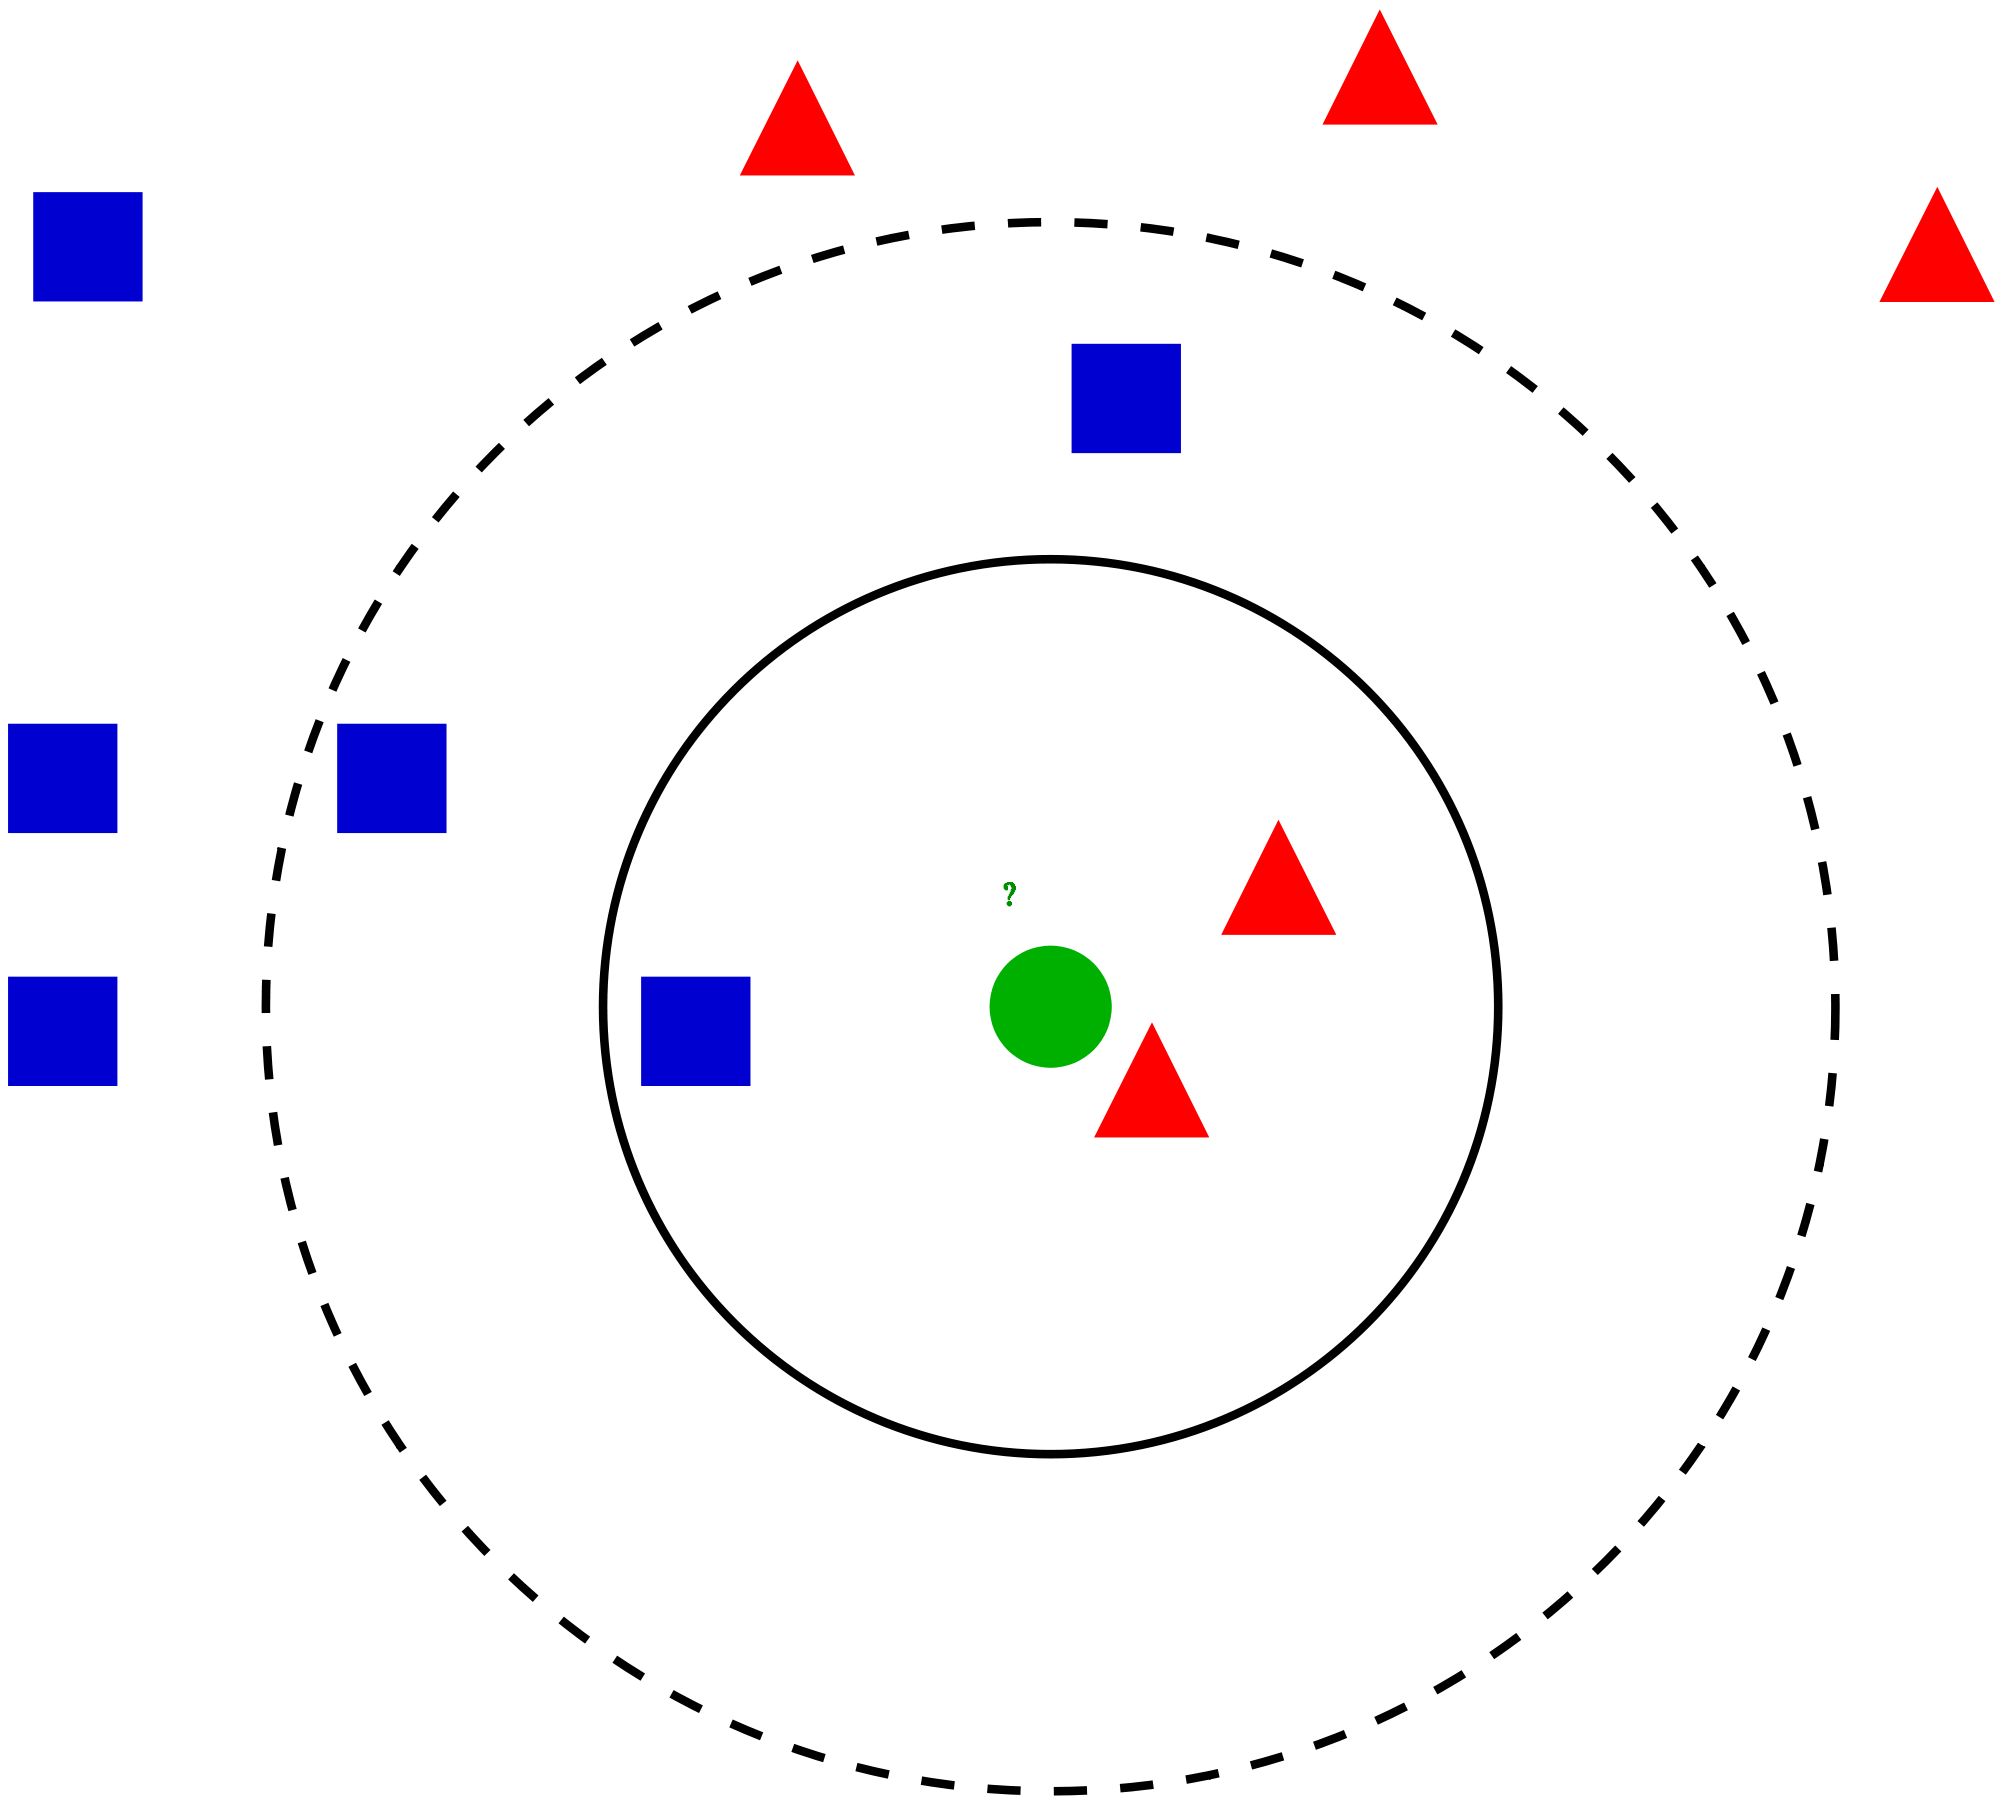
\includegraphics[width=\columnwidth]{bilder/2000px-KnnClassification.jpg}
    \end{center}
    \caption{kNN-klassificering av den runda observationen i mitten i ett rum
    med två klasser, trianglar och kvadrater. Majoritetsomröstning
    med $k=3$ leder till att den runda klassas som triangel, medan $k=5$ leder
    till klassificering som kvadrat. \copyright Antti Ajanki, 2007}
    \label{fig:knn-overview}
\end{figure}

\end{document} 

